\documentclass[hidelinks, 12pt, a4paper]{article}

\usepackage[utf8]{inputenc}
\usepackage[margin=1.5cm]{geometry}
\usepackage{graphicx}
\usepackage{setspace}
\usepackage[T1]{fontenc}
\usepackage{tocloft}
\usepackage{todonotes}
\usepackage{epstopdf} 
\usepackage{hyperref}
\usepackage{float}
\usepackage{titlesec}
\usepackage{listings}
\usepackage{multirow}
\usepackage{xcolor}
\usepackage{mwe}
\usepackage{hyperref}
\onehalfspacing
\usepackage[english]{babel}
\usepackage{fancyhdr}
\usepackage{enumitem}

\pagestyle{fancy}
\fancyhf{}
\rhead{blulancetech@gmail.com}
\lhead{Carpool}
\rfoot{Page \thepage}

\author{}
\date{}
\title
{
	
\includegraphics[width=6cm]{images/up_logo.jpg} \\
	Department of Computer Science \\
	Faculty of Engineering, Built Environment \& IT\\
	University of Pretoria \\
	\vspace{0.5cm}
	\Huge COS301 -
	Software Engineering\\
	\vspace{1cm}
	{\Huge Carpool}\\
	\begin{Large}
	Carpool Coding standards document
	\end{Large}
	\vspace{0.5cm}
	
    \begin{center}
    \noindent
    
\includegraphics[width=6cm]{images/company_logo.png} 
    \vspace{0.5cm}
    \begin{table}[h]
    \centering
    \begin{tabular}{|l|l|l|}
    \hline
    Name  & Student Number\\ \hline
    Benjamin Osmers & u16068344 \\ \hline
    Ashleigh Govender &  U20528834      \\ \hline
    Joshua Brink  & U19185678 \\ \hline
    Jason Antalis     & U19141859     \\ \hline
    Wesley Pachai & U20578688    \\ \hline
            
    \end{tabular}
    \end{table}
    \end{center}
    }

\begin{document}
\maketitle


\newpage
\tableofcontents
\newpage
\section{Introduction}

    The goal of this paper is to lay out the coding guidelines for the Carpool Application. It ensures that our code has a consistent style, is clear, flexible, reliable, and efficient.
   \vspace{1cm} 
\section{Naming Conventions}

  When it comes to naming conventions, the following guidelines should be followed:
    
       \subsection{\large{\textbf{Classes:}}}
        \begin{itemize}[]
            \item When naming our classes we made use of camel Casing - If the class consisted of two words, the first letter of the first word would be lower case and the first letter of the second word would be uppercase.
            \item If the name of our class was more then two words, we did not have spaces or underscores between them, we just differentiated the beginning and end of the world using uppercase and lowercase.
        \end{itemize}
        
        \vspace{0.5cm} 
        
         \subsection{\large{\textbf{Function headers and Variables:}}}
        \begin{itemize}[]
            \item  For front end functions we capitalised the first letter of each word, and for back-end functions we used camel casing.
            \item  For both front-end and back-end, we used lower case variables except in the case of ENUMS, or constants. In this case we capitalised the entire word. In testing when we made use of mock variables, we used camel case.
        \end{itemize}
        
         \vspace{0.5cm} 
        
         \subsection{\large{\textbf{Schema:}}}
        \begin{itemize}[]
            \item  When naming attributes in the schema, we made use of Camel case.
            \item If the attribute was two words, we did not use a space or a underscore, we just differentiated the beginning and end of the world using uppercase and lowercase.e.g userId
            \item ENUM attributes are named using Capital letters
            \item  When naming tables in the schema, we made use of Pascal case.
            \item If the table name was two words, we did not use a space or a underscore, we just differentiated the beginning and end of the world using uppercase and lowercase.e.g PickUpLocation.
            \item No two tables are named the same.
        \end{itemize}
        
\newpage
        
\section{Repository Branching Structure}
\subsection{Branching}
Since we split the coding aspect of this project into use cases. Each member of the group creates a branch with their name, whether they are working client side or back end side(API, database), and exactly what use case/ feature they are working on. .The format of branching will be as follows: name/category/feature. Meaning category may have three options, namely: client, api, db.For example "jason/client/bookseat" is a vaild branch. These branches are then periodically merged into the main branch by another member of the team once it as passed the CI tests and the other member has reviewed the changes
\vspace{0.2cm} 
\begin{center}
    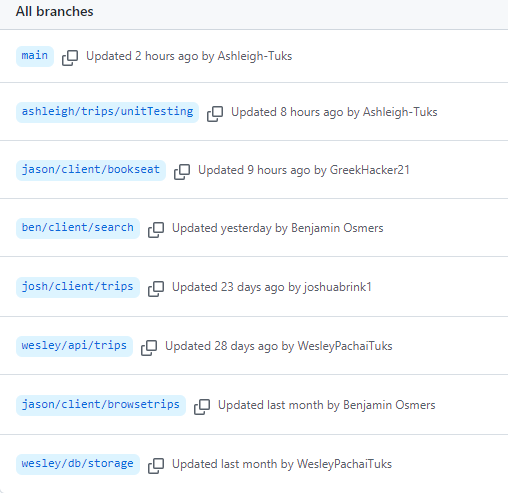
\includegraphics[width=6cm]{images/Branching.png} \\
\end{center}
\vspace{0.5cm} 

\subsection{Pull Requests and Commits}
Commits will need to have detailed naming along with a suitable gitmoji to help describe what has been done within that commit.
Every pull request has to pass the CI tests and has to be reviewed by another member of the group before it is merged into the main branch.  The person who made the pull request cannot merger their branch to the main branch.
\vspace{0.5cm} 
\newpage
\subsection{Repository Structure}
Below is a screenshot of our repository structure, at the top we have all our code and files, and towards the bottom of the page we have links to our documentation as well as a brief bio on every member in the group
\begin{center}
    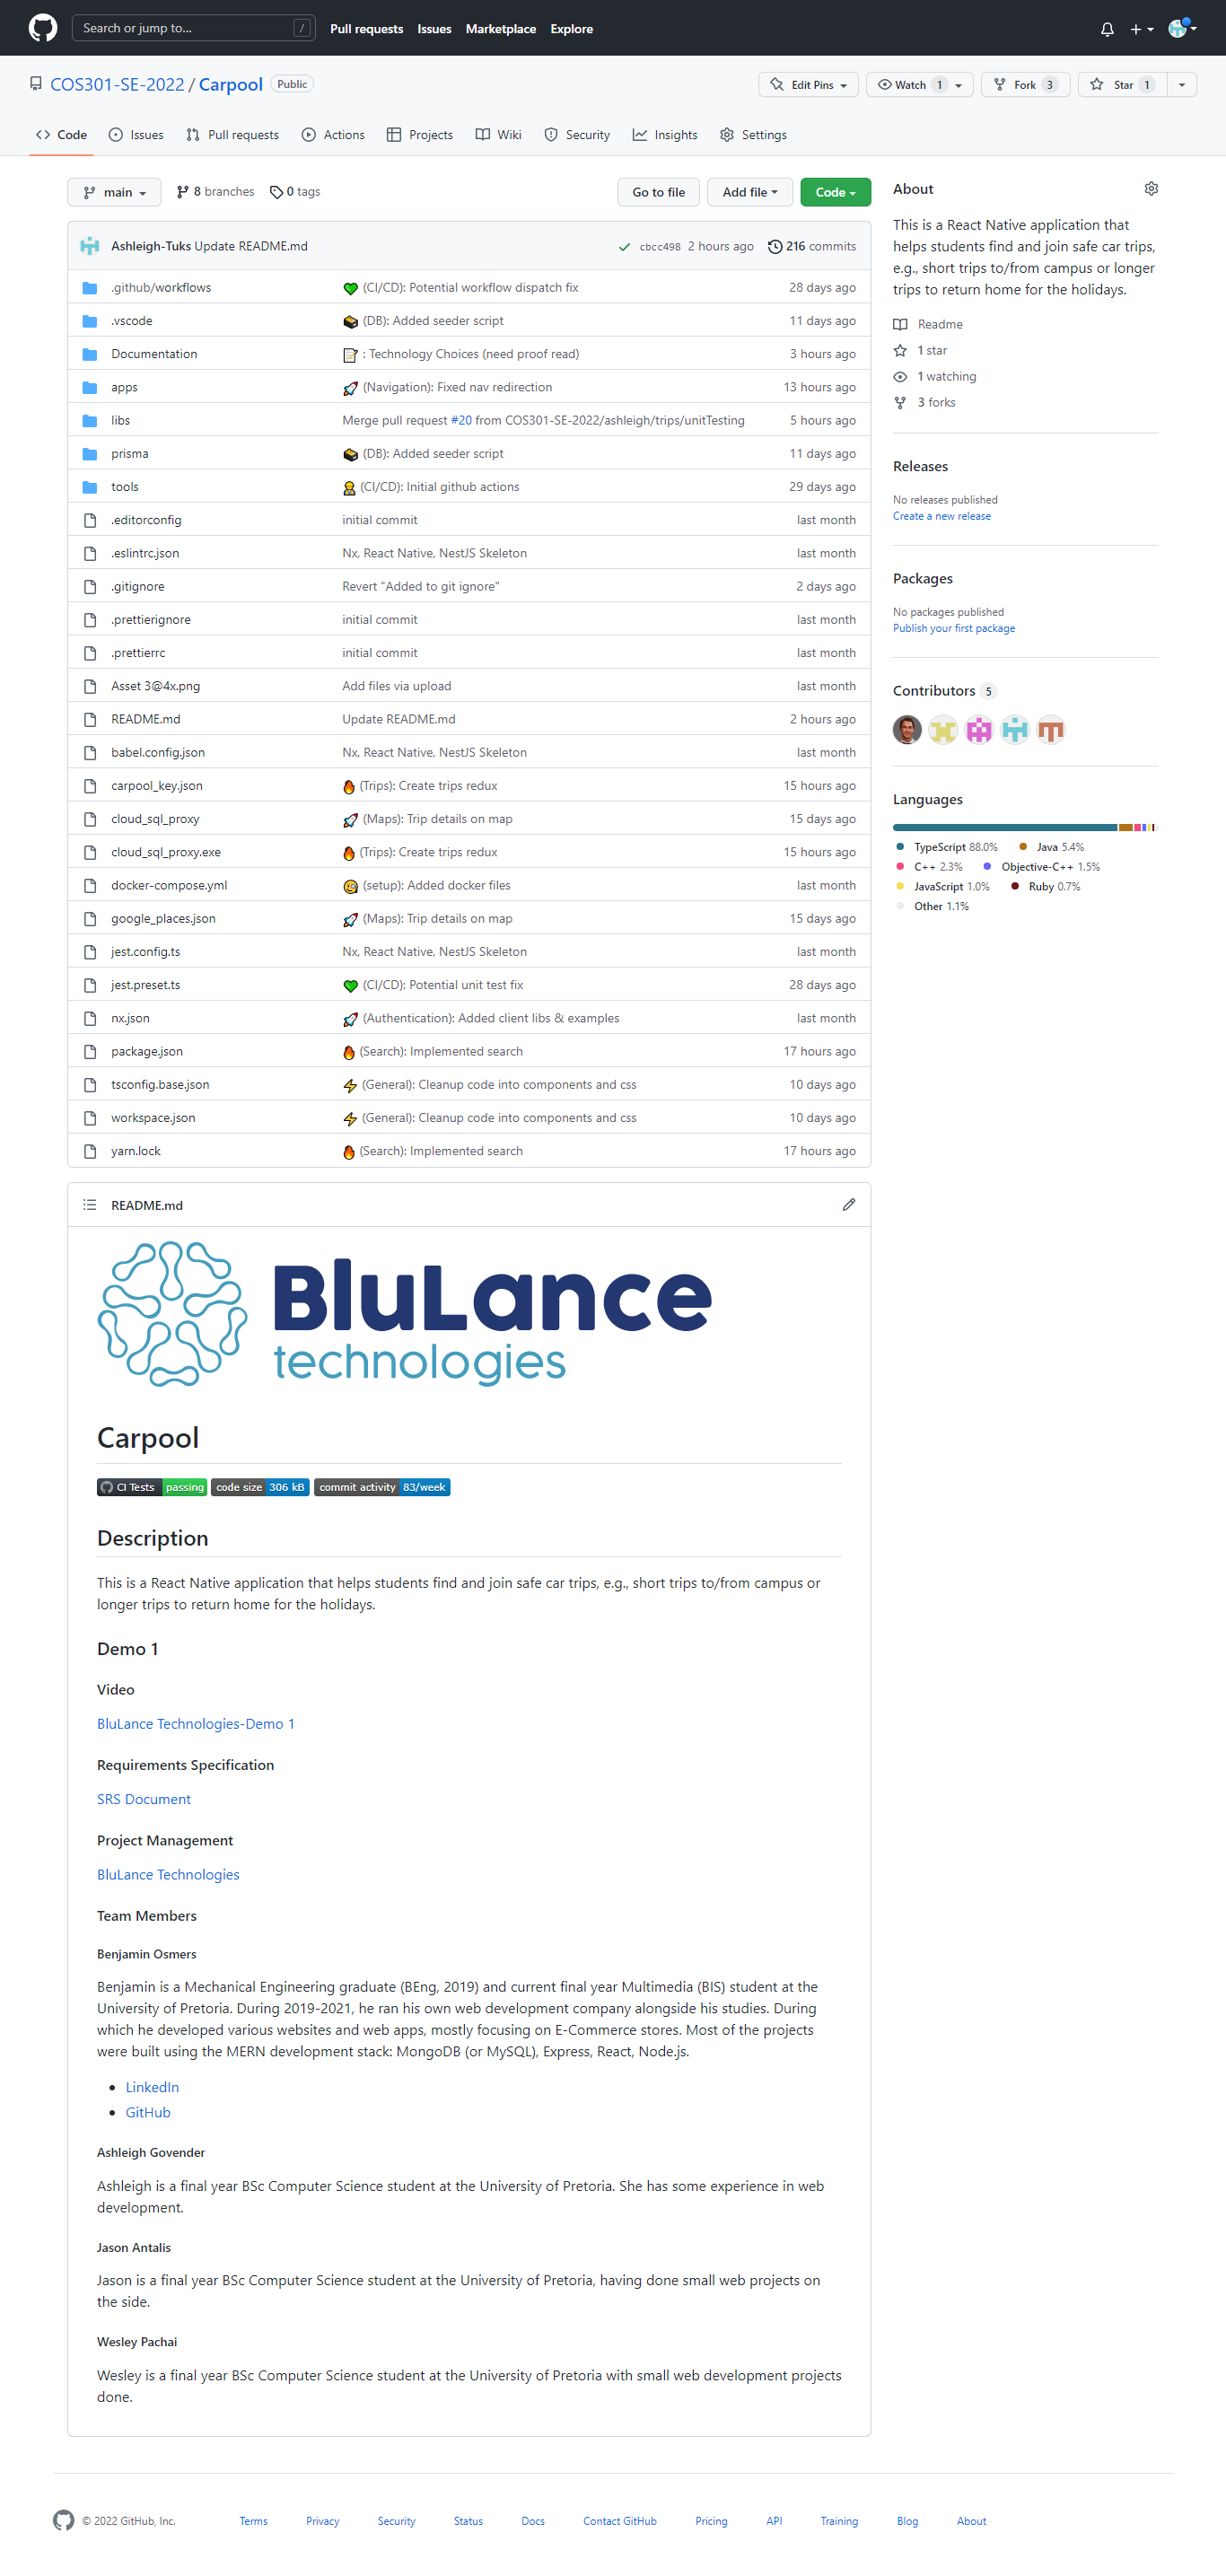
\includegraphics[width=6cm]{images/GitHub.png} \\
\end{center}
\vspace{0.5cm} 

\newpage  

\section{Comments}
    
        When Adding comments code the following principles will be used:\\
        
        Single Line Comments:
        \begin{code}
         \begin{lstlisting}
         /* Insert comment about code */   
        // Insert comment about code
         \end{lstlisting}
       \end{code}
       
        multi-line comment:
         \begin{code}
    
        \begin{lstlisting}
        /** 
        * Comment spreads across multiple lines
        * This could be used for large comments.
        */
        \end{lstlisting}
            
        \end{code}               
 

        function header comment:
            
        \begin{code}
        
        \begin{lstlisting}
        /** 
        * Describe what the function does
        * 
        * @param parameterName- brief over view of each parameter passed into the function
        * 
        * @return a short description of what the function returns.
        */
        \end{lstlisting}
        \end{code}
\newpage

\section{File Structure}
Our system is broken up into front-end and back-end. Our file structure represents that split.
\begin{center}
    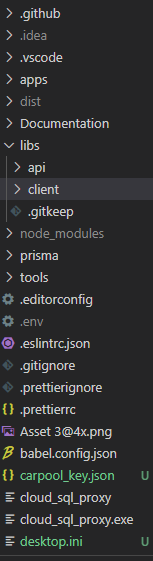
\includegraphics[width=6cm]{images/File Structure 1.png} \\
\end{center}
\vspace{0.5cm} 
Back-end can be found at libs/API where as front-end can be found at libs/Client 
\newpage Back-end is further split up into API, Service and Repository layers.
\begin{center}
    \includegraphics[width=6cm]{images/File Structure 3.png} \\
\end{center}
\vspace{0.5cm} 
Each of these layers have their own spec.ts (usually used for unit testing) file and .ts files(resolver, data access, service)
\begin{center}
    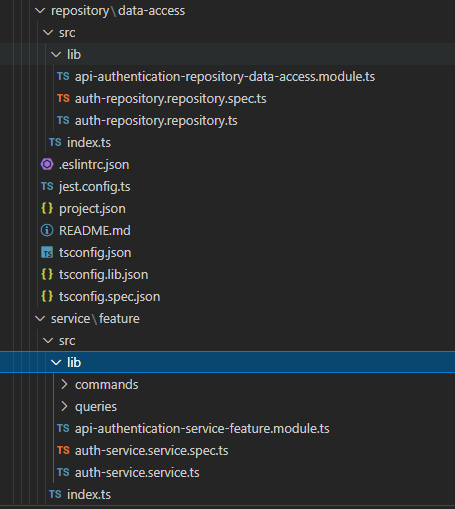
\includegraphics[width=6cm]{images/File Structure 5.png} \\
\end{center}
\vspace{0.5cm} 
The front-end splits the pages, store and componments up.
\begin{center}
    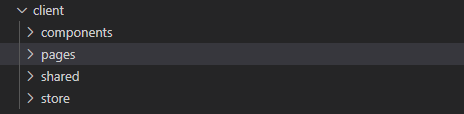
\includegraphics[width=6cm]{images/File Structure 6.png} \\
\end{center}
\vspace{0.5cm} 

\end{document}